\documentclass{article}
\usepackage{arxiv}

\usepackage[utf8]{inputenc}
\usepackage[english, russian]{babel}
\usepackage[T1]{fontenc}
\usepackage{url}
\usepackage{booktabs}
\usepackage{amsfonts}
\usepackage{nicefrac}
\usepackage{microtype}
\usepackage{lipsum}
\usepackage{graphicx}
\usepackage{natbib}
\usepackage{doi}
\usepackage{amsmath}



\title{Spatiotemporal forecasting with convolutionals and tensor decomposition}

\author{ Max Gorishniy \\
	Phystech School of Applied Mathematics and Computer Science\\
	Moscow institute of physics and technology\\
	Mosow \\
	\texttt{gorishnii.mp@phystech.edu} \\
	%% examples of more authors
	\And
	Nadezhda Alsahanova \\
	Moscow institute of physics and technology \\
	Moscow \\
	\texttt{alsahanova.nyu@phystech.edu} \\
	\And
	Vadim Strijov \\
	Moscow institute of physics and technology \\
	Moscow \\
	\texttt{strijov@phystech.edu} \\
}
\date{}

\renewcommand{\shorttitle}{\textit{arXiv} Template}

%%% Add PDF metadata to help others organize their library
%%% Once the PDF is generated, you can check the metadata with
%%% $ pdfinfo template.pdf
\hypersetup{
pdftitle={Spatiotemporal forecasting with convolutionals and tensor decomposition},
pdfauthor={Max Gorishniy, Nadezhda Alsahanova, Vadim Strijov},
pdfkeywords={SSA, TSSA, time series reconstruction},
}

\begin{document}
\maketitle

\begin{abstract}
Tensor based time series decomposition methods based on singular spectrum analysis showed great results in both denoising and interpretability. Several forecasting techniques based on them were already explored, yet none provided simultaneously accurate, stable and computationally cheap inferring. After an in-depth study of well known models we facilitated a new one comprising all three requirements for non-stationary quasi-periodic time series. The model was then tested on real-life data of electricity consumption and other well-explored datasets. 
\end{abstract}


\keywords{SSA \and TSSA \and time series reconstruction}

\section{Introduction}
Singular spectrum analysis (SSA) is a method widely used in the past decades in different areas, from economics to biology and social science \cite{golyandina2020}.  One of main advantages is its ability to extract underlying frequencies from complex and multidimensional data, resulting in  variable number of components. SSA consists of two main stages: decomposition and reconstruction, both adjustable in terms of methods and hyperparameters used.

Its modification, tensor singular spectrum analysis (TSSA) \cite{kouchaki2013}, offers a more robust and accurate results by converting a series into a tensor and using  parallel factor analysis (PARAFAC) decomposition instead of the usual SVD. It optimizes usage of information initially available to a model in cost of working with more multidimensional data SSA does. The problem of reconstruction is left untouched however.

Empirical mode decomposition (EMD) can then be used  to supervise TSSA, giving us TSSA-EMD \cite{kouchaki2015}. It provides a better way to identify the number of frequency components within each subspace. With such enhancement algorithms achieves \cite{kouchaki2015} a distinguishable growth in accuracy of signal reconstruction with denoising, leaving other methods far behind in particular tasks.

Basic SSA shows \cite{golyandina2020} adequate results when working with series of constant-limited variation function. However it becomes highly unstable in two basic cases. With several outliers already false frequencies are extracted at decomposition stage, what does not lead to reconstruction defects but enforces unacceptable error even at earlier points of prediction. A variation growth affects SSA the same way, usually creating frequencies of much higher amplitude than are expected. That makes the early predictions seem accurate, yet giving unrealistic forecast long-wise.

To conclude, SSA is a powerful but limited method.

At the same time SSA does not utilize spatial information. Given a set of parallel time series it is meant to decompose each separately. TSSA instead can show better performance by working with them as with a whole dataset. Knowing this we experiment to determine the difference between SSA and TSSA forecasting and try to create a robust model of signal decomposition, reconstruction and prediction.
\section{Problem}
\label{sec:Problem}

\subsection{Time series}

Let \(x = \left[x_1, x_2, ..., x_n\right]\), \(x_i \in \mathbb{R}\) be a 1D time series, namely a vector. We suppose \(x\) has no trend, is quasi-periodic and it's phase trajectory is stationary.

\subsection{Hankelization}

One of the SSA steps requires Hankelization operator \(\mathcal{H}\) to be described. With 2D matrix \(i \times j\) it works as follows:
\begin{gather}
\mathcal{H}M =
\begin{pmatrix}
	\widetilde{m}_{1} & \widetilde{m}_{2} & \dots & m_{i} \\
	\widetilde{m}_{2} & \widetilde{m}_{3} & \dots & m_{i + 1} \\
	\vdots & \vdots & \ddots & \vdots \\
	\widetilde{m}_{j} & \widetilde{m}_{j + 1} &  \dots & \widetilde{m}_{i + j - 1}
\end{pmatrix} \notag \\
\widetilde{m}_{k} = \sum_{i, j \in D_k} m_{i,j} / numD_k \\
D_k = \{(\widehat{i}, \widehat{j}) : 1 \leq \widehat{i} \leq i, 1 \leq \widehat{j} \leq j, \widehat{i} + \widehat{j} = k + 1\} \notag
\end{gather} 
For a  higher dimensional tensor \(\mathcal{H}\) performs first index wise.

\subsection{SSA}

The basic SSA consists of two stages. The first is decomposition, it maps time series to a number of components. The second is reconstruction, it combines components to frequencies of interest.

Decomposition: given a 1D vector \(x\) of size \(n\) and window size \(l\) it first creates a 2D embedding of it, a trajectory matrix \(X\) of size \(l_x \times l\):
\begin{gather}
X = [X_1, X_2, ..., X_{l}] = \mathcal{H} x = 
 \begin{pmatrix}
	x_{1} & x_{2} & \dots & x_{l} \\
	x_{2} & x_{3} & \dots & x_{l + 1} \\
	\vdots & \vdots & \ddots & \vdots \\
	x_{l_{x}} & x_{l_x + 1} &  \dots & x_{l_x + l - 1}
\end{pmatrix} \notag \\
l_x = n - l + 1
\end{gather}

The actual value of \(l\) is chosen arbitrarily to include enough information about the signal variance.

Singular value decomposition (SVD) is then applied to \(X\) to obtain its singular values and vectors:

\begin{gather}
X = \sum \limits_{i = 1}^{d} X_i = \sum \limits_{i = 1}^{d} \sqrt{\lambda_i} u_i v_i^T
\end{gather}

Where \( \lambda_i \) is the \(i\)th eigenvalue, \(u_i\) is the corresponding left singular vector and \(v_i\) is the \(i\)th right singular vector; \(d\) is the total number of eigenvalues.

Reconstruction: given a set of components \(X_i\) it first splits them into disjoint set and sums independently:

\begin{gather}
I = \{ I_1, I_2, \dots, I_q \}, \bigsqcup \limits_{i = 1}^{q} I = \{1, 2, \dots, d\} \notag \\
X = \sum \limits_{i = 1}^{q} \hat{X}_i = \sum \limits_{i = 1}^{q} \sum \limits_{j \in I_i} X_j
\end{gather}

The choice of I is one of the most important aspects of SSA in terms of retrieving the desired frequencies. \(X_i\) are considered base frequencies for the initial time series. First \(k\) of them are then taking as a basis for the reconstruction. The rest are discarded.

Inverse hankelization is then applied to \(\sum_{i=1}^{k}X_i\) by taking mean of secondary diagonal elements, resulting in a reconstructed time series \(\hat{x}\).

% \begin{gather}
% \hat{x} = \sum \limits_{i = 1}^{l_x} \sum \limits_{j = 1}^{l} \hat{X}_{i,j} / l_x, l_x = n - l + 1
% \end{gather}

\subsection{TSSA}

TSSA is a generalization of SSA to work with a set of parallel time series. It is based on the assumption that parallel time serieses are not independent and that the information contained in one of them can be used to improve the general reconstruction error. 

PARAFAC decomposition is used to decompose the tensor of time series into a set of components in Khatri-Rao form, sorted by their contribution to the reconstruction error. First \(k\) components are then taken and summed to form the reconstructed after Khatri-Rao form being unreaveled to a final tensor.

\section{SSA and TSSA comparison, algorithm}

SSA with window width \(l\) is taken as a baseline, with optimum \(l\) found by gridsearch for each particular dataset.

For TSSA the time series is first converted into matrix by disjoint windowing:

\begin{gather}
X = [X_1, X_2, ..., X_{m}] =
 \begin{pmatrix}
	x_{1} & x_{2} & \dots & x_{m} \\
	x_{m+1} & x_{m+2} & \dots & x_{2m} \\
	\vdots & \vdots & \ddots & \vdots \\
	x_{k_{x}+1} & x_{k_x + 2} &  \dots & x_{k_x + m}
\end{pmatrix} \text{, }
k_x = \lfloor \frac{n}{m} \rfloor
\end{gather}

Where the hyperparameter \(m\) is gridsearched for each dataset to lower the resulting reconstruction error.

The matrix is then Hankelized with window width \(l\) and the PARAFAC is applied to it, resulting in a set of components in Khatri-Rao form. They are then sorted by an individual loss optimization so that the components are in the order of decreasing importance.

For both SSA and TSSA the first-\(k\) reconstruction loss is calculated for each \(k\). Area under curve (AUC) is then calculated for the loss curves and the method with the lowest AUC is chosen as the best for a dataset.

As a standalone solution a TSSA with both \(m\) and \(l\) gridsearched to achive the best results. Compared to SSA, TSSA is computationally expensive, but more information about a time series as whole is saved in each local area inside a hankelized matrix, giving it more opportunities to find the best reconstruction. Its ability to utilize spatial information also makes it applicable to a set of parallel time series, which is not possible with SSA. This results in a better reconstruction error and higher robustness.

For a real-time application TSSA hyperparameters are estimated on a training set and then used for a suffix of a particular time series realization.

\section{Experiment}

Thought different data exploration multiple reconstruction strategies were tested: first-k SSA, first-k TSSA, [katrutsa-isachenko]. Means squared error (MSE) was used as a measure of error, minimizing it is an optimization task for which optimum method is to be found. Several synthetic time series were generated to test the methods. Then the real data of electricity consumption was used to test the methods.

We use \(f(t) = \sin(\pi t) + np.sin(et)\) for \(t \in (0, 100)\), sampling it uniformly to \(100\) points to create a time series. The data generated looks as follows:

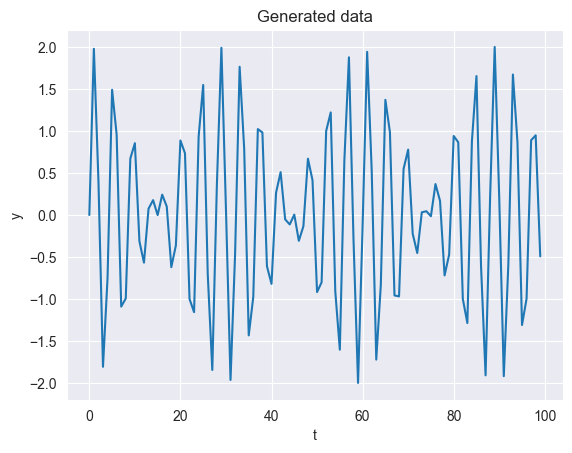
\includegraphics[scale=0.7]{./images/fig1.png}

SSA is then applied with different numbers of components taken at reconstruction step. The results for log-MSE error for window size 5 are as follows:

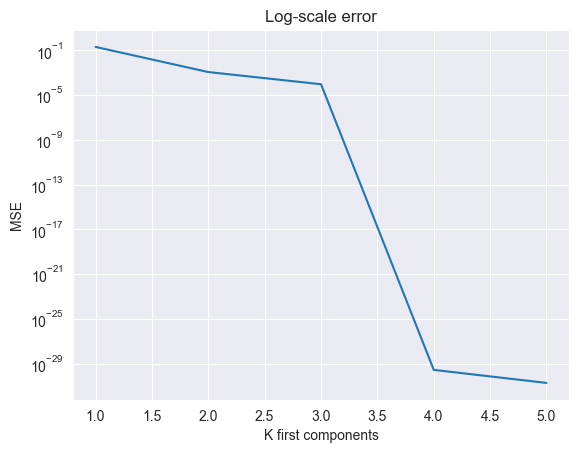
\includegraphics[scale=0.7]{./images/fig2.png}

With first 4 components taken at reconstruction step the error is non-significant already. More complex data must be taken to see the difference when applying PARAFAC.

\section{Real data experiments}

Example of the experiment on a real-data time series is described here: usage of first-k SSA reconstruction, hankelization of the data and PARAFAC decomposition for it. The results on different datasets are listed in the end.

Electricity consumption dataset consists of 8760 samples - one for each hour of the year. For SSA it is given with window size 24, acquiring that number of base frequencies. For each \(k \in [1, 24]\) components are then summed and a reconstruction error MAPE is calculated. For PARAFAC the data is hankelized and then decomposed into Khatri-Rao form with \(k = 24\) components. Same prefix sum operation is applied to the components and the reconstruction error is calculated. The results are shown on the figure below.

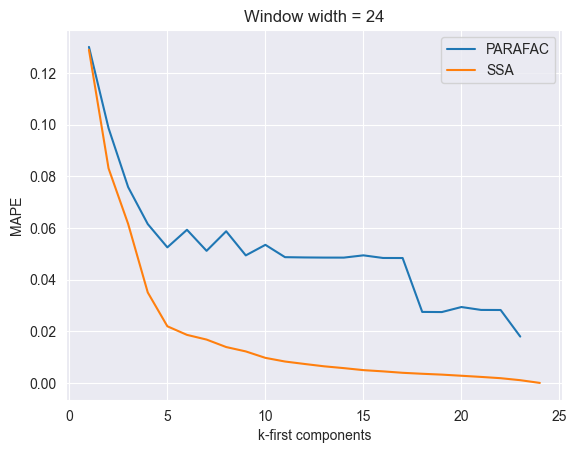
\includegraphics[scale=0.7]{./images/fig3.png}

% \begin{table}
% 	\caption{MAPE comparison on real data.}
% 	\centering
% 	\begin{tabular}{c|c}
% 		\toprule
% 		% \multicolumn{2}{c}{Part}                   \\
% 		% \cmidrule(r){1-2}
% 		Method     & Dataset (series length) \\
% 		\midrule
% 		First-k SSA  & Input terminal  \\
% 		First-k TSSA & Output terminal \\
% 		     & Cell body       \\
% 		\bottomrule
% 	\end{tabular}
% 	\label{tab:table}
% \end{table}


% \section{Trash}

% \subsection{Citations}
% Citations use \verb+natbib+. The documentation may be found at
% \begin{center}
% 	\url{http://mirrors.ctan.org/macros/latex/contrib/natbib/natnotes.pdf}
% \end{center}

% Here is an example usage of the two main commands (\verb+citet+ and \verb+citep+): Some people thought a thing \citep{kour2014real, hadash2018estimate} but other people thought something else \citep{kour2014fast}. Many people have speculated that if we knew exactly why \citet{kour2014fast} thought this\dots

% \subsection{Figures}
% \lipsum[10]
% See Figure \ref{fig:fig1}. Here is how you add footnotes. \footnote{Sample of the first footnote.}
% \lipsum[11]

% \begin{figure}
% 	\centering
	
% 	\caption{Sample figure caption.}
% 	\label{fig:fig1}
% \end{figure}

% \subsection{Tables}
% See awesome Table~\ref{tab:table}.

% The documentation for \verb+booktabs+ (`Publication quality tables in LaTeX') is available from:
% \begin{center}
% 	\url{https://www.ctan.org/pkg/booktabs}
% \end{center}


% \begin{table}
% 	\caption{Sample table title}
% 	\centering
% 	\begin{tabular}{lll}
% 		\toprule
% 		\multicolumn{2}{c}{Part}                   \\
% 		\cmidrule(r){1-2}
% 		Name     & Description     & Size ($\mu$m) \\
% 		\midrule
% 		Dendrite & Input terminal  & $\sim$100     \\
% 		Axon     & Output terminal & $\sim$10      \\
% 		Soma     & Cell body       & up to $10^6$  \\
% 		\bottomrule
% 	\end{tabular}
% 	\label{tab:table}
% \end{table}

% \subsection{Lists}
% \begin{itemize}
% 	\item Lorem ipsum dolor sit amet
% 	\item consectetur adipiscing elit.
% 	\item Aliquam dignissim blandit est, in dictum tortor gravida eget. In ac rutrum magna.
% \end{itemize}


% \bibliographystyle{unsrtnat}
% \bibliography{references}

\section{Conclusion}

SSA and TSSA both are powerful methods for time series analysis. They can extract interpretable frequencies and reconstruct a denoised series of them. SSA is computationally cheap and is easier to setup, but it is not able to utilize spatial information. TSSA is computationally expensive, but on certain datasetsets with proper parameters choice can achieve better reconstruction error. In the future it is planned to create more optimal algorithm for the choice of TSSA parameters so it could achive lowest error for a particular dataset without gridsearch or manual parameter tuning.

\nocite{*}
\bibliographystyle{unsrt}
\bibliography{references}

\end{document}